%%%%%%%%%%%%%%%%%%%%%%%%%%%%%%%%%%%%%%%%%%%%%%%%%%%%%%%%%%%%%
%%  Introduction											%
%%%%%%%%%%%%%%%%%%%%%%%%%%%%%%%%%%%%%%%%%%%%%%%%%%%%%%%%%%%%%

\section{Introduction}

%-------	Computational approaches	-------%
	Computational studies of organs and bioprosthetic devices have become increasingly popular for predicting the outcomes of diseases, injuries, and surgical interventions. Such applications include the simulation of aneurysm growth \cite{rissland_abdominal_2009,ramault_comparison_2011,hoi_effects_2004,volokh_model_2008}, blood flow \cite{olufsen_numerical_2000,perktold_computer_1995,pries_blood_1990,oshima_finite_2001,bagchi_mesoscale_2007}, and natural or bioprosthetic heart valves \cite{zakerzadeh_computational_2017, soares_biomechanical_2016, kamensky_immersogeometric_2015, aggarwal_vivo_2016, nobili_numerical_2008, cheng_three_2004}. One of the most important components of predictive simulations is an accurate constitutive model that can predict the mechanical behavior of the soft tissues and biomaterials involved. Such tissues exhibit nonlinear anisotropic behaviors, often resulting in highly specific forms for different tissue types. In addition, these constitutive models are often extended to model growth, remodeling, pathology, fatigue, trauma and other time evolving processes. As such, complex constitutive models are often developed to take advantage the structure to function relationship to predict how the response of the material will evolve, utilizing physical models of the tissue microstructure, multi-scale approaches, and/or molecular dynamics. Not surprisingly, constitutive models are becoming exceeding complex, and the computational costs are becoming a hindrance to more complex numerical simulations. 


%-------	structural modeling	-------%
	One example of such approach are meso-scale structural approaches for soft tissue modeling \cite{lanir_constitutive_1983}. This class of soft tissue models homogenize the tissues at the meso-scale, where the simplified models of the mechanical response of collagen, elastin and other fibers are integrated with tissue microstructure \cite{kassab_structure_2016}. This type of constitutive model has been shown to be able to accurately represent the mechanical behaviors of many tissues including valvular tissues \cite{zhang_meso_2016, rego_mitral_2016}, pericardium \cite{zhang_modeling_2017}, myocardium \cite{avazmohammadi_novel_2017}, and elastomeric scaffolds \cite{d.amore_large_2016}. Recently,
we have extended these models to include interaction terms \cite{zhang_modeling_2017} \cite{avazmohammadi_novel_2017}, which require multiple integrals to accurately compute the strain energy of fiber interactions. 




%-------	multi-scale modeling	-------%
    In a broader context, multi-scale approaches utilize fundamental mechanisms at the micro-scale to derived the response of a material at the macro-scale. Often, multi-scale modeling begins at the molecular level, where the molecular structure of the constituents of the material and the physical laws governing their interactions are well known and well-studied in chemistry and physics. At this level, molecular dynamics can be used to determine the mechanical response of constituent proteins. This can be upscaled further for quaternary protein structures using coarse grain methods. This response is then integrated with higher level structures of the tissue to determine the response at even larger scales. Homogenization is thus critical in multi-scale modeling to simplify and smooth over the heterogeneities in the response of the downscale models to improve the efficient of simulations at a higher scale. This process is repeated until reaching the macro-level. Examples using this approach is the modeling of collagenous tissues by Buehler \textit{et al.} \cite{buehler_atomistic_2006, buehler_nanomechanics_2008} and intermediate filament of cells by Qin \textit{et al.} \cite{qin_multi_2010}. 
    
    
    However, numerical simulations using this approach is also quite costly, can only be used for simulating the response of the material, and cannot be easily incorporated into inverse modeling and time-dependent frameworks. Even the resulting computational cost of meso-scale structural approaches is five magnitudes higher than conventional phenomenological approaches. For more detailed cell or molecular level information, which are important for better understanding cellular environments and growth and remodeling, the exceedingly high computational cost of multi-scale approaches makes it difficult to be directly implemented in computational simulations. As such, the multi-scale models used in simulations need to be simplified.

%-------	modeling material behavior	-------%
    It is for this reason that many types of phenomenological models with computationally efficient forms, such as the generalized Fung type \cite{fung_biomechanics_1993}, Holzapfel-Gasser-Ogden \cite{holzapfel_new_2000}, generalized Ogden \cite{ogden_large_1972}, generalized Rivlin \cite{rivlin_large_1951}, and Humphrey models \cite{may-newman_constitutive_1998}, are popular for numerical simulations. These models utilize constitutive modeling approaches which do not take into account of the underlying mechanisms, thus can only match the mechanical response in the limited range of experimental data utilized for parameter estimation. Furthermore, the mechanical data used and parameter estimation are done in an optimal manner. This makes reaching optimal parameters inconsistent due to high covariance often found between parameters. This is demonstrated in Sun and Sacks \cite{sun_biaxial_2003} for modeling pericardium under high in-plane shear. Here, it was shown that fitting only a subset of the loading paths acquired from biaxial mechanical testing cannot predict the remaining unfitted loading paths. Yet for \textit{in vivo} simulations, these constitutive models are often derived from incomplete data while being asked to predict the mechanical response under non-physiological and often unpredictable ranges of deformation. As the parameters of such models have no physical meaning, it is often difficult to not possible to extend them for time dependent processes such as growth and remodeling, or even averaged to produce a population representative. As such, accurate simulations often still require detailed mechanism based models. 
    

%-------	effective model	-------%
    To address these problems, an approach which can taking advantage of mechanisms and predictive capabilities of micro-models (meso-scale, multi-scale, or other complex constitutive models) and the numerical efficiency of phenomenological approaches for simulations at the macro-scale is very beneficial. An effective constitutive model, based on phenomenological approaches, can be used to accurately reproduce the responses of a wide range of tissues using the same form, acting as an intermediate step between micro-models for material behavior and organ-level numerical simulations (Fig. \ref{fig:simulationframework}A). For each iteration of the simulation, whether forward, inverse, or time-evolving, the effective constitutive model is first fit to the micro-model(s) to determine the model parameters, then it is used to performed the actual numerical simulation. Subsequent updates to the evolving material properties, geometry and boundary conditions are then performed (Fig. \ref{fig:simulationframework}B). This makes the effective constitutive models especially useful for the final upscaling step of multi-scale models, increasing their efficiency. However, developing a generalized effective constitutive model is not straight forward. In addition to the issues described above, no specific constitutive model has yet been developed that is able to capture the material response of a wide range of soft tissue responses. Typically, a different constitutive model is used for each soft tissue type. These issues remain to be reconciled if effective constitutive models are to be used to reliably and fully reproduce the response of micro-models in computational simulations. 
    
    Thus, we hereby develop an effective constitutive model for planar soft tissues, and a parameter estimation approach for rapidly determining the model parameters from the micro-model. Planar constitutive models is a good starting point, applicable to a wide range of soft tissues such as arteries, skin, heart valve, cells, vocal folds, bladder wall, synovial membrane, cornea, and cranial membrane. For the form of the effective constitutive model, we require the following characteristics:
\begin{enumerate}
    \item Widely applicable in that it is able to faithfully reproduce a wide range of tissue responses
    \item Low computational cost, efficient, and numerically robust
    \item Allows for fast and accurate convergence during parameter estimation for upscaling micro-models, thus having the minimal number of and minimally covariant model parameters
    \item Easy to implement, no integrations or functions without closed-form expressions
\end{enumerate}
Using meso-scale structural models as an example, we will examine the ability of the effective constitutive model to fit the mechanical response of micro-models for a wide range of deformations, examine the speed and convergence of parameter estimation, and demonstrate the use of the effective constitutive model to facilitate the simulation of heart valves with a wide range of material properties.
    
%%%%%%%%%%%%%%%%%%%%%%%%%%%%%%%%%%%%%%%%%%%%%%%%%%%%%%%%%%%%
%-------------------	begin FIGURE 	-------------------%
\begin{figure}
\centering
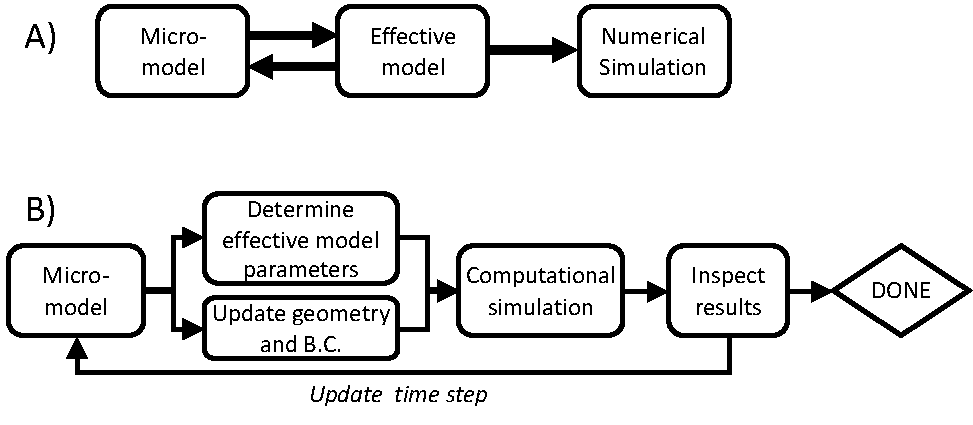
\includegraphics[width=6.5in]{Figures/simulationframework}
\caption{Proposed frame work for using an effective constitutive model to improve the efficiency of using complex meso- or multi-scale models (micro-models) in numerical simulations. Here, A) effective constitutive models act as an intermediate step between micro-models and numerical simulations, where micro-models inform the changes to the effective constitutive model while the effective constitutive model for the simulation. B) An example of how this may be implemented for time-evolving is shown.}
\label{fig:simulationframework}
\end{figure}
%-------------------	 end FIGURE 	-------------------%
%%%%%%%%%%%%%%%%%%%%%%%%%%%%%%%%%%%%%%%%%%%%%%%%%%%%%%%%%%%%
    
    
    
    
    
    
    
    
